\section{Classes and Objects}

In this section a breakdown of the main classes and objects used in the system architecture is provided. Each class is described in terms of its attributes, methods, and relationships with other classes.

\subsection{Resource AAS classes}
In this subsection a detailed breakdown of the classes representing the AAS-Agent interface , the BDI agent Layer and the defnition of the Submodels .

\newpage
\subsubsection{Submodels definition}
In this subsection is the definition of the submodels of the Resource AAS.
Figure \ref{fig:submodel_classes} shows the class diagram representing the Resource Submodel, while Table \ref{tab:submodels_overview} provides an overview of each submodel along with its elements and definitions.
\begin{figure}[ht]
    \centering
    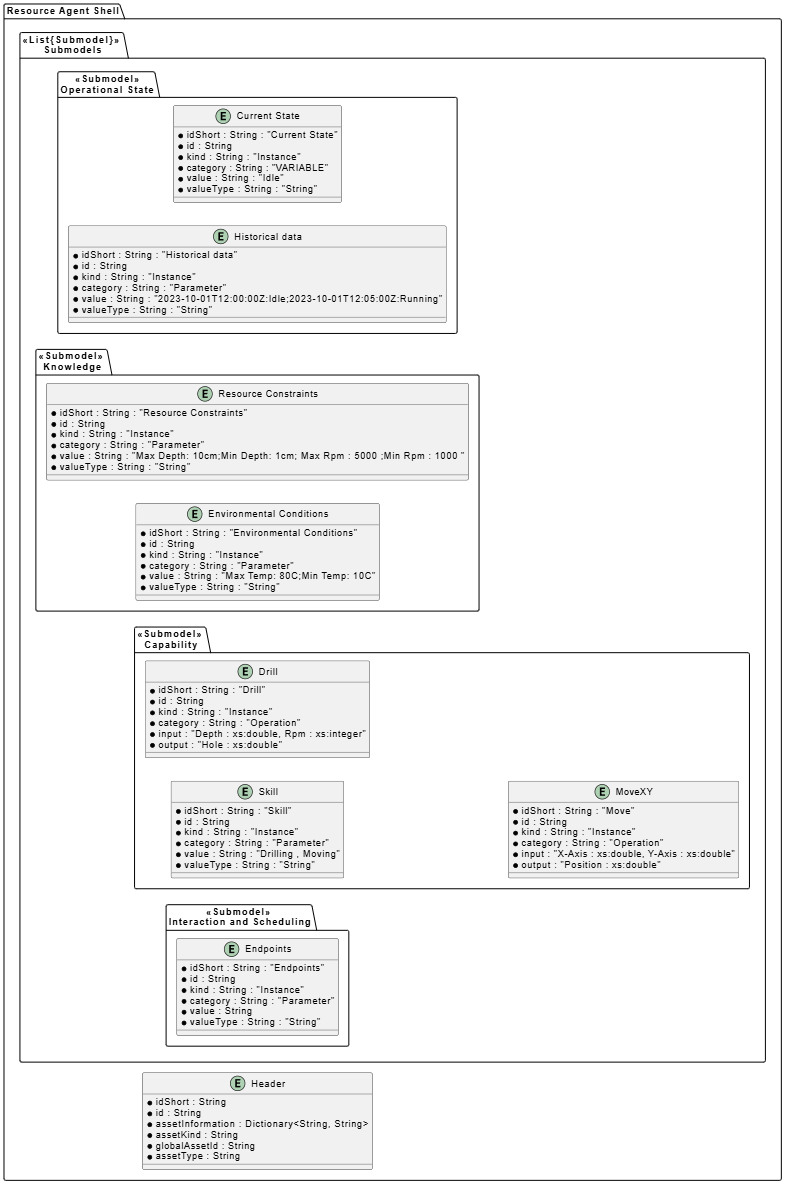
\includegraphics[width=0.7\textwidth]{Images/Classes_Resource/Submodels/Submodels.png}
    \caption{Class diagram representing the Resource Submodel.}
    \label{fig:submodel_classes}
\end{figure}
\begin{table}[ht]
  \centering
  \caption{Overview of Resource Submodels and their elements}
  \label{tab:submodels_overview}
  \begin{tabularx}{\textwidth}{|l|X|X|}
    \hline
    \textbf{Submodel} & \textbf{Elements} & \textbf{Definition / Purpose} \\
    \hline
    Operational State & Current State , Historical Data & Represents the current and historical operational states of the resource. \\
    \hline
    Knowledge & Resource Constraints, Environmental Conditions & Contains knowledge about resource constraints and environmental conditions affecting operations. \\
    \hline
    Capability & Drill , MoveXY ,Skill & Defines the capabilities and skills of the resource for task execution. \\
    \hline
    Interaction and Scheduling & Endpoints & Manages interaction points and scheduling information for resource coordination. \\
    \hline
  \end{tabularx}
\end{table}

\newpage
\subsubsection{REST Client}
This subsection provides a detailed breakdown of the classes representing the REST Client used for communication with the AAS.
Figure \ref{fig:rest_client_classes} shows the class diagram representing the REST Client.
\begin{figure}[ht]
    \centering
    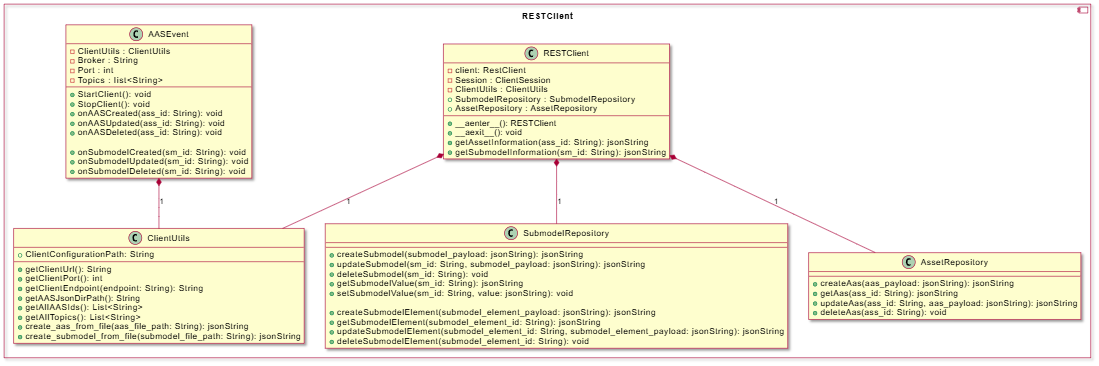
\includegraphics[width=0.9\textwidth]{Images/Classes_Resource/REST_Client.png}
    \caption{Class diagram representing the REST Client.}
    \label{fig:rest_client_classes}
\end{figure}

The main design of this component is the two repository classes, the \emph{AAS Repository} class that is responsible for all the communication with the AAS over REST API calls, and the \emph{Submodel Repository} class that is responsible for all the communication with a specific submodel of the AAS over REST API calls.
Both classes use the \emph{HTTP Client} class that is a wrapper over the HTTP library used to perform the REST API calls.
Those then are called into the main class \emph{REST Client} that creates, starts, and stops a client session.
Also the class provides a simple MQTT client to subscribe to AAS events over MQTT protocol.
This client is represented by the \emph{AASEvent} class.

\newpage
\subsubsection{AAS-Agent Interface}
This subsection provides a detailed breakdown of the classes representing the AAS-Agent interface.
Figure \ref{fig:aas_agent_interface_classes} shows the class diagram representing the AAS-Agent Interface.
\begin{figure}[ht]
    \centering
    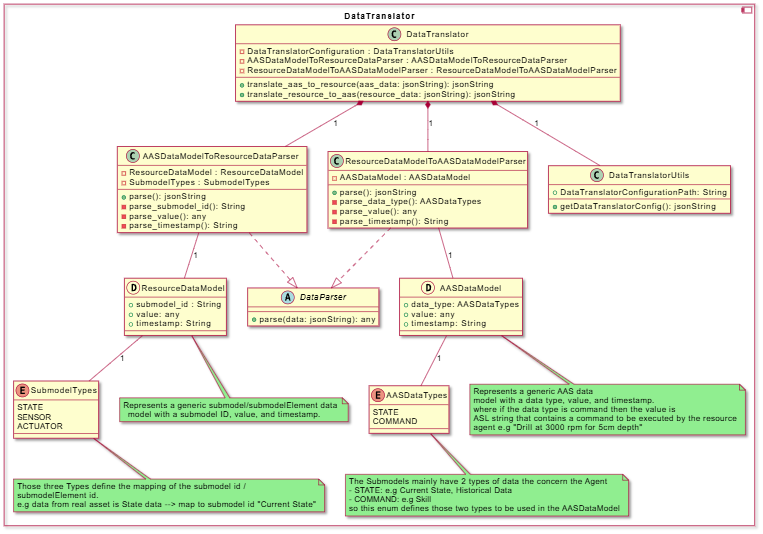
\includegraphics[width=0.8\textwidth]{Images/Classes_Resource/DataTranslator.png}
    \caption{Class diagram representing the AAS-Agent Interface.}
    \label{fig:aas_agent_interface_classes}
\end{figure}

This interface provides the needed datatypes to switch between the data coming from the AAS and the data coming from the Resource Asset over the agent.
The datatype that represent the data coming from the AAS to the agent is the \emph{AAS Data Model} class, while the datatype that represent the data coming from the Resource Asset to the agent is the \emph{Resource Data Model} class.
This conversion is done through the \emph{DataParser} class that is an abstract class that contains the methods needed for the conversion between the two datatypes.
The \emph{AAS to Resource Data Parser} class is a concrete implementation of the \emph{DataParser} class that implements the conversion from the \emph{AAS Data Model} to the \emph{Resource Data Model}, while the \emph{Resource to AAS Data Parser} class is a concrete implementation of the \emph{DataParser} class that implements the conversion from the \emph{Resource Data Model} to the \emph{AAS Data Model}.
Finally the \emph{Data Translator} is the main level that is callable through entry points from the BDI agent layer to perform the needed conversion between the two datatypes.
In the lowest level there is two enums  the \emph{AAS Data Types} enum that contains the data types used in the AAS Data Model and the \emph{Resource Data Types} enum that contains the data types used in the Resource Data Model.

\newpage
\subsubsection{BDI Agent Core}
This subsection provides a detailed breakdown of the classes representing the BDI Agent Core.
Figure \ref{fig:bdi_agent_core_classes} shows the class diagram representing the BDI Agent Core.
\begin{figure}[ht]
    \centering
    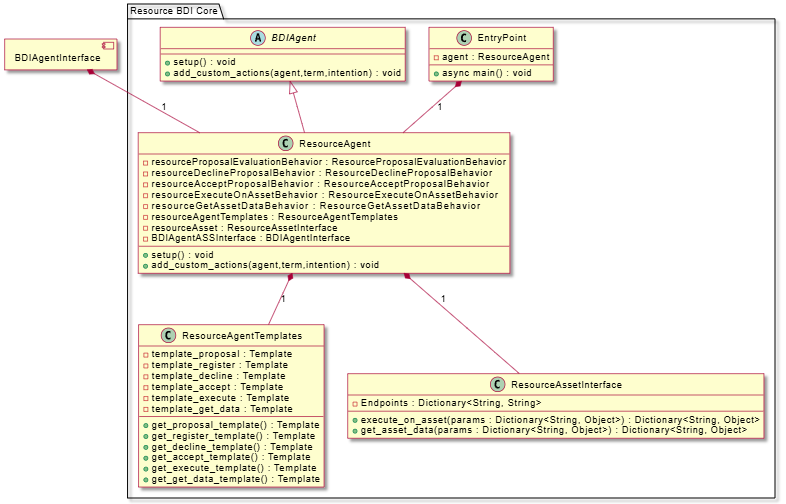
\includegraphics[width=0.9\textwidth]{Images/Classes_Resource/BDI_Core/Agent_core.png}
    \caption{Class diagram representing the BDI Agent Core.}
    \label{fig:bdi_agent_core_classes}
\end{figure}

By using \textbf{SPADE} framework , there is an architecture that represents the BDI agent core.
Mainly each agent core contians an Agent core where the BDI Agent lives and Behaviours that represent the different functionalities of the agent.
In the figure \ref{fig:bdi_agent_core_classes} is the Agent Core represented ,while in figure \ref{fig:bdi_agent_behaviours_classes} are the different behaviours of the agent represented.
\begin{figure}[ht]
    \centering
    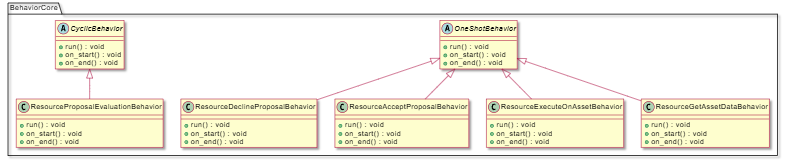
\includegraphics[width=0.95\textwidth]{Images/Classes_Resource/BDI_Core/Behaviours.png}
    \caption{Class diagram representing the BDI Agent Behaviours.}
    \label{fig:bdi_agent_behaviours_classes}
\end{figure}

The \emph{ResourceAgent} class is the main class that represents the BDI agent.
Its mainly an implementation of the \textbf{SPADE} \emph{BDIAgent} class.
The needed methods to be implemented are the \emph{setup} method that is called when the agent is started and the \emph{add custom actions} that let the agent define action or desires that is represtented in the behaviours.
The Data exchange between the agents in the \textbf{SPADE} framework is done mainly throgh \textbf{Templates} which are represented by the \emph{Resource Agent Templates} class.
The Behaviours of the agent is represented by two abstract classes of the \textbf{SPADE} framework: \emph{OneShotBehaviour} and \emph{CyclicBehaviour}.
Those then are implemented into different concrete classes like the \emph{Proposal Process Behaviour} class that is responsible for handling the proposals coming from the Orchestrator agent, the \emph{Task Execution Behaviour} class that is responsible for executing the tasks assigned to the resource, and the \emph{Status Update Behaviour} class that is responsible for updating the status of the resource in the AAS at regular intervals.

\newpage
\subsection{Production AAS classes}
This subsection provides a detailed breakdown of the classes representing the Production AAS-Agent interface , the Orchestrator Layer and the definition of the Submodels.

\subsubsection{Submodels definition}

In this subsection is the definition of the submodels of the Production AAS.
Figure \ref{fig:prod_submodel_classes} shows the class diagram representing the Production Sub
model, while Table \ref{tab:prod_submodels_overview} provides an overview of each submodel along with its elements and definitions.
\begin{figure}[ht]  
    \centering
    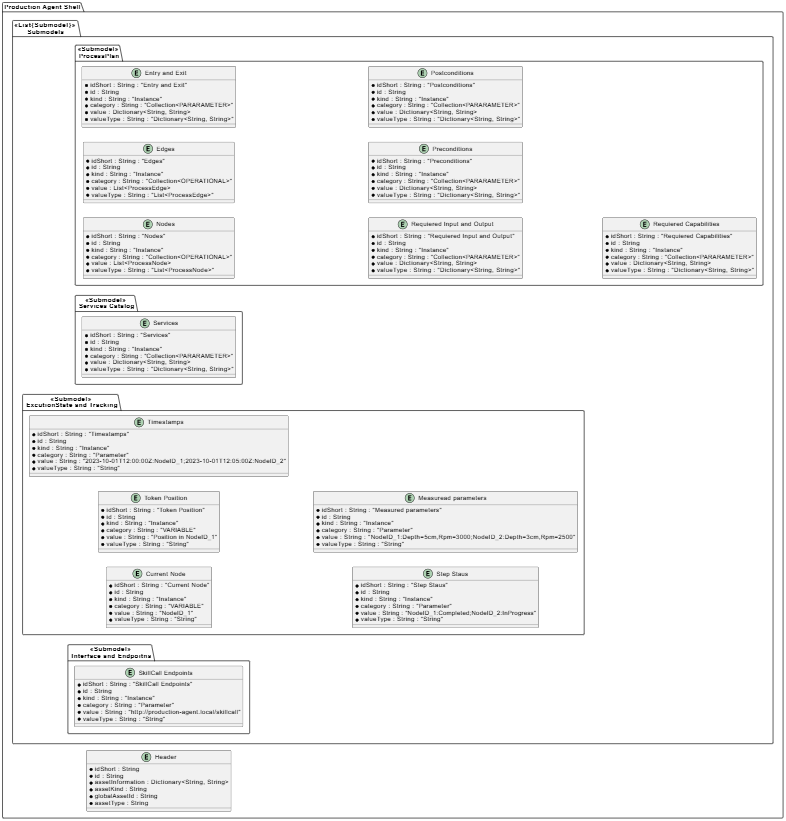
\includegraphics[width=0.7\textwidth]{Images/Production_Classes/Submodels.png}
    \caption{Class diagram representing the Production Submodel.}
    \label{fig:prod_submodel_classes}
\end{figure}

\begin{center}
\begin{longtable}{|p{0.18\textwidth}|p{0.41\textwidth}|p{0.41\textwidth}|}
\caption{Overview of Production Submodels and their elements}
\label{tab:prod_submodels_overview}\\
\hline
\textbf{Submodel} & \textbf{Elements} & \textbf{Definition / Purpose} \\
\hline
\endfirsthead
\multicolumn{3}{c}{\tablename\ \thetable\ -- \textit{Continued from previous page}} \\
\hline
\textbf{Submodel} & \textbf{Elements} & \textbf{Definition / Purpose} \\
\hline
\endhead
\hline \multicolumn{3}{r}{\textit{Continued on next page}} \\
\endfoot
\hline
\endlastfoot
Process Plan & Entry \& Exit; Nodes; Edges; Preconditions; Postconditions; Required Input \& Output; Required Capabilities. & Defines the procedural/workflow model for a production task. Nodes represent steps, edges represent transitions; pre/postconditions control applicability; inputs/outputs and required capabilities describe data and resources needed by each step. Used for orchestration and execution planning. \\
\hline
Services Catalog & Services (service id, signature, parameters, category). & Registry of callable services / functional capabilities exposed by the production component. Describes available service operations, required parameters and invocation metadata for integration and discovery. \\
\hline
Execution State \& Tracking & Timestamps; Token position; Current node; Step status; Measured parameters. & Runtime information about process execution and monitoring: timestamps and token positions for traceability, current node and step status for progress reporting, measured parameters for quality/telemetry. Enables tracking, auditing and recovery. \\
\hline
Interface and Endpoints & SkillCall Endpoints (URIs / endpoint descriptors). & Communication and integration endpoints used to invoke skills or services remotely (e.g., orchestrator calls, skill invocation). Contains addressing and protocol metadata for external interaction. \\
\hline
Header / Metadata & idShort, id, administration/asset information, semantic identifiers, versioning. & Global AAS header and identification information that links the submodel to the asset and provides administrative metadata (identifiers, semantic references and versioning). Used for discovery and semantic alignment. \\
\hline
\end{longtable}
\end{center}

\newpage
\subsubsection{REST Client}
Similar to the Resource AAS REST client, this subsection provides a detailed breakdown of the classes representing the REST Client used for communication with the Production AAS.
Figure \ref{fig:prod_rest_client_classes} shows the class diagram representing the REST Client.
\begin{figure}[ht]
    \centering  
    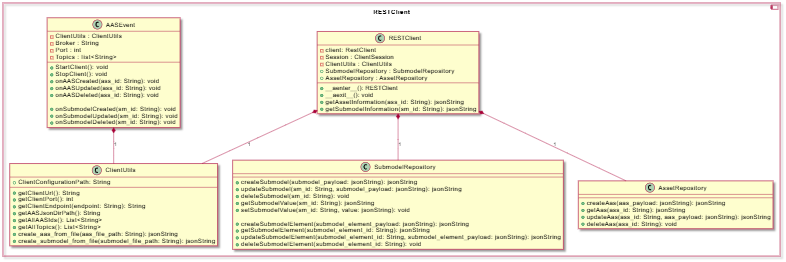
\includegraphics[width=0.99\textwidth]{Images/Production_Classes/Client.png}
    \caption{Class diagram representing the REST Client.}
    \label{fig:prod_rest_client_classes}
\end{figure}
The design of this component is similar to the Resource AAS REST client, with two repository classes: the \emph{Production AAS Repository} class for communication with the Production AAS over REST API calls, and the \emph{Production Submodel Repository} class for communication with specific submodels of the Production AAS over REST API calls.
Both classes utilize the \emph{HTTP Client} class for performing REST API calls.
The main class \emph{REST Client} creates, starts, and stops a client session, and also provides an MQTT client to subscribe to Production AAS events over the MQTT protocol, represented by the \emph{ProductionAASEvent} class.


\newpage
\subsubsection{AAS-Agent Interface}
This subsection provides a detailed breakdown of the classes representing the Production AAS-Agent interface.
Figure \ref{fig:prod_aas_agent_Translator_classes} shows the class diagram representing the Production AAS-Agent Interface.
\begin{figure}[ht]
    \centering  
    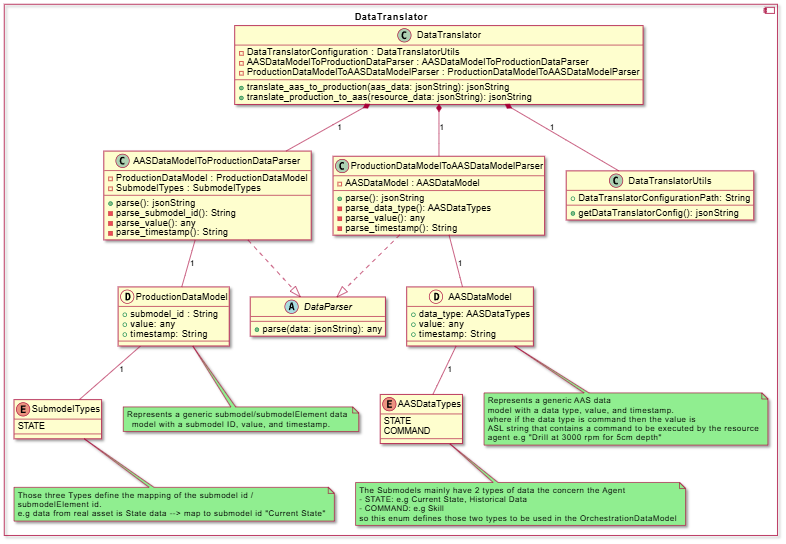
\includegraphics[width=0.8\textwidth]{Images/Production_Classes/Translator.png}
    \caption{Class diagram representing the Production AAS-Agent Interface.}
    \label{fig:prod_aas_agent_Translator_classes}
\end{figure}

The main diffrerence between this interface and the Resource AAS-Agent interface is the datatypes used.
The datatype that represent the data coming from the Production AAS to the Orchestrator agent is the \emph{Production AAS Data Model} class, while the datatype that represent the data used internally by the Orchestrator agent is the \emph{Production Data Model} class.
This conversion is done through the \emph{Production DataParser} class that is an abstract class that contains the methods needed for the conversion between the two datatypes.
The \emph{Production AAS to Production Data Parser} class is a concrete implementation of the \emph{Production DataParser} class that implements the conversion from the \emph{Production AAS Data Model} class to the \emph{Production Data Model} class.
The Interface is showen in figure \ref{fig:prod_aas_agent_interface_classes}.
\begin{figure}[ht]
    \centering  
    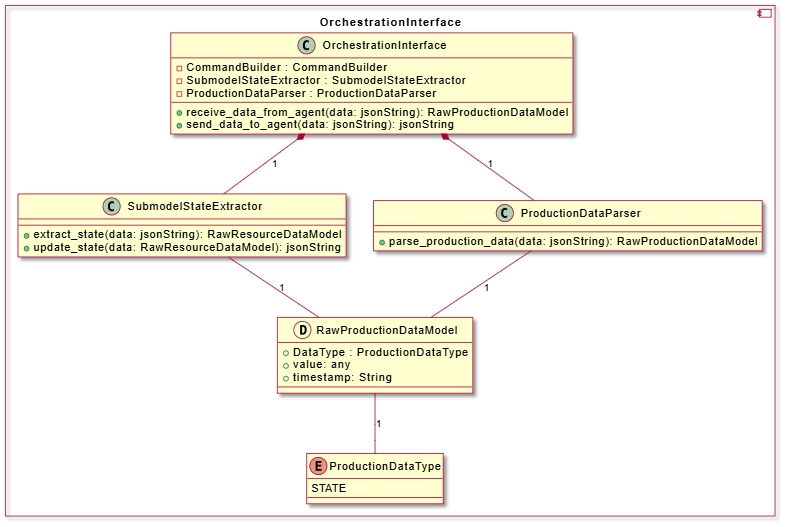
\includegraphics[width=0.8\textwidth]{Images/Production_Classes/Interface.png}
    \caption{Class diagram representing the Production AAS-Agent Interface.}
    \label{fig:prod_aas_agent_interface_classes}
\end{figure}

\newpage
\subsubsection{Orchestration and Negotiation Core}

This subsection provides a detailed breakdown of the classes representing the Orchestration and Negotiation Core.
The orchestration Core is represented in figure \ref{fig:orchestration_core_classes}.
\begin{figure}[ht]
    \centering  
    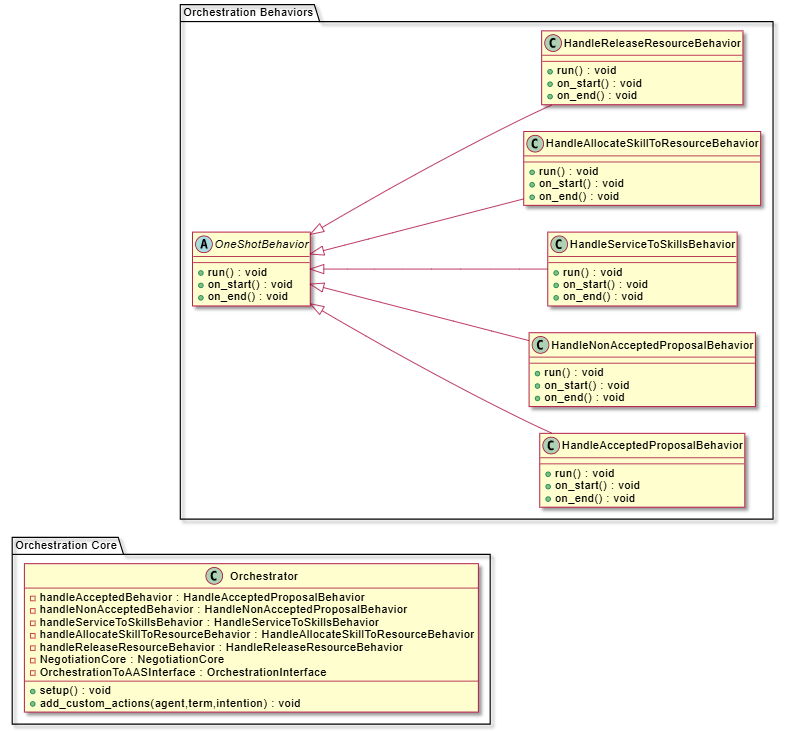
\includegraphics[width=0.9\textwidth]{Images/Production_Classes/Agent_Core/Orch_Core.png}
    \caption{Class diagram representing the Orchestration Core.}
    \label{fig:orchestration_core_classes}
\end{figure}
The Orchstrator is the main class that represents the Orchestrator agent.
Its mainly an implementation of the \textbf{SPADE} \emph{Agent} class.
The needed methods to be implemented are the \emph{setup} method that is called when the agent is started and the \emph{add custom actions} that let the agent define action or desires that is represtented in the behaviours.
The Data exchange between the agents in the \textbf{SPADE} framework is done mainly throgh \textbf{Templates} which are represented by the \emph{Orchestrator Agent Templates} class.
The Behaviours of the agent is represented by an abstract classe of the \textbf{SPADE} framework: \emph{OneShotBehaviour}.
Those then are implemented into different concrete classes like the \emph{Allocate Skill To Resource Behaviour} class that is responsible for allocating skills to resources based on their capabilities, and the \emph{Negotiation Behaviour} class that is responsible for handling the negotiation process with Resource agents to finalize task assignments.

The other core which is the Negotiation core is represented in figure \ref{fig:negotiation_core_classes}.
This is also represented by and Agent class in the \textbf{SPADE} framework.
It also have defined behaviours that are represented in the figure. \ref{fig:negotiation_core_classes}.
\begin{figure}[ht]
    \centering
    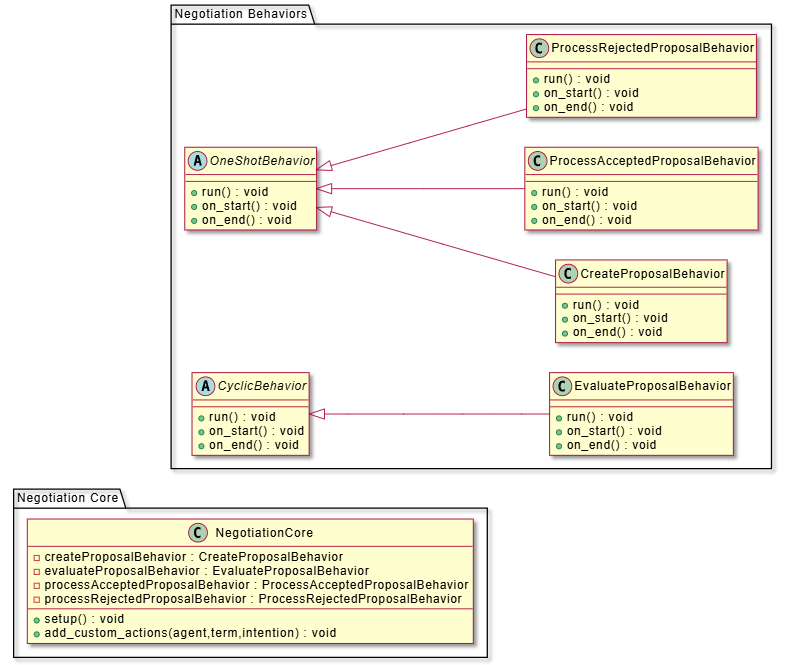
\includegraphics[width=0.9\textwidth]{Images/Production_Classes/Agent_Core/Negotiation_Core.png}
    \caption{Class diagram representing the Negotiation Core.}
    \label{fig:negotiation_core_classes}
\end{figure}

The two cores work together to manage the orchestration of production tasks and the negotiation with Resource agents to ensure optimal task assignments based on resource capabilities and time availability.

